% begin module arccos-properties
\begin{frame}
Important facts about $\Arccos$:
\begin{columns}[c]
\column{.5\textwidth}
\psset{xunit=1.2cm,yunit=1.2cm}
\begin{pspicture}(-1.9,-0.5)(1.9,3.8)
\tiny
\psaxes[labels=none, ticks=none] {<->}(0,0)(-1.8,-0.5)(1.8,3.7)
\psLabels{1.8}{3.7}
\psline(1,-0.1)(1,0.1)
\psplot[linecolor=red, plotpoints=1000]{-1}{1}{x ACOS}
\psline(-0.1,3.141592654)(0.1,3.141592654)
\rput[l](0.15,3.141592654){$\pi$}
\psline(-1,-0.1)(-1,0.1)
\rput[t](-1,-0.1){$-1$}
\rput[t](1,-0.1){$1$}
\rput[r](-0.6, 2){$y=\Arccos x$}
\uncover<handout:0| 3>{
\psline[arrows=<->, linecolor=red, linewidth=3pt](-1,0)(1,0)
} 
\uncover<handout:0| 5>{
\psline[arrows=<->, linecolor=red, linewidth=3pt](0,0)(0,3.141592654)
} 
\end{pspicture}

%\ 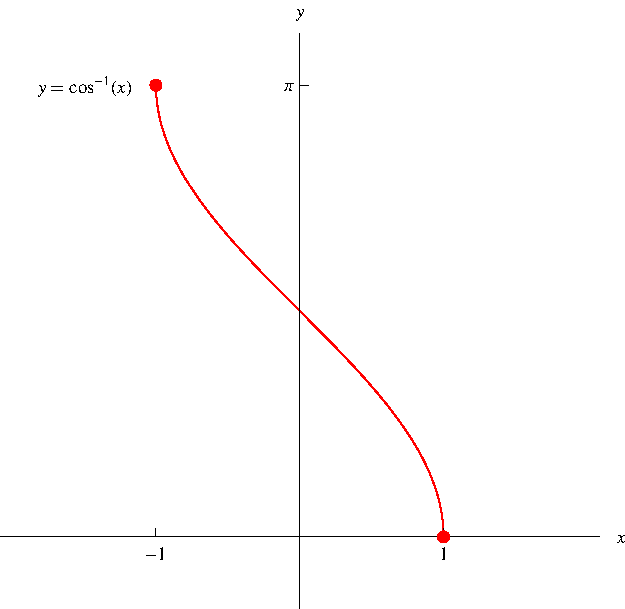
\includegraphics[height=6cm]{inverse-trig/pictures/07-06-arccosd.pdf}%
\column{.5\textwidth}
\begin{enumerate}
\item  \alert<handout:0| 2-3>{Domain: \uncover<3-| handout:0>{$[-1, 1]$.}}
\item  \alert<handout:0| 4-5>{Range: \uncover<5-| handout:0>{$[0, \pi ]$.}}
\item  $\Arccos x = y \Leftrightarrow \cos y = x$ and $0 \leq y \leq \pi$.
\item  $\Arccos (\cos x) = x$ for $0 \leq x \leq \pi$.
\item  $\cos (\Arccos x) = x$ for $-1 \leq x \leq 1$.
\item  $\frac{\diff}{\diff x} (\Arccos x) = -\frac{1}{\sqrt{1-x^2}}$.  \uncover<6->{(The proof is similar to the proof of the formula for the derivative of $\Arcsin x$.)}
\end{enumerate}
\end{columns}
\end{frame}
% end module arccos-properties
